\documentclass[1p]{elsarticle_modified}
%\bibliographystyle{elsarticle-num}

%\usepackage[colorlinks]{hyperref}
%\usepackage{abbrmath_seonhwa} %\Abb, \Ascr, \Acal ,\Abf, \Afrak
\usepackage{amsfonts}
\usepackage{amssymb}
\usepackage{amsmath}
\usepackage{amsthm}
\usepackage{scalefnt}
\usepackage{amsbsy}
\usepackage{kotex}
\usepackage{caption}
\usepackage{subfig}
\usepackage{color}
\usepackage{graphicx}
\usepackage{xcolor} %% white, black, red, green, blue, cyan, magenta, yellow
\usepackage{float}
\usepackage{setspace}
\usepackage{hyperref}

\usepackage{tikz}
\usetikzlibrary{arrows}

\usepackage{multirow}
\usepackage{array} % fixed length table
\usepackage{hhline}

%%%%%%%%%%%%%%%%%%%%%
\makeatletter
\renewcommand*\env@matrix[1][\arraystretch]{%
	\edef\arraystretch{#1}%
	\hskip -\arraycolsep
	\let\@ifnextchar\new@ifnextchar
	\array{*\c@MaxMatrixCols c}}
\makeatother %https://tex.stackexchange.com/questions/14071/how-can-i-increase-the-line-spacing-in-a-matrix
%%%%%%%%%%%%%%%

\usepackage[normalem]{ulem}

\newcommand{\msout}[1]{\ifmmode\text{\sout{\ensuremath{#1}}}\else\sout{#1}\fi}
%SOURCE: \msout is \stkout macro in https://tex.stackexchange.com/questions/20609/strikeout-in-math-mode

\newcommand{\cancel}[1]{
	\ifmmode
	{\color{red}\msout{#1}}
	\else
	{\color{red}\sout{#1}}
	\fi
}

\newcommand{\add}[1]{
	{\color{blue}\uwave{#1}}
}

\newcommand{\replace}[2]{
	\ifmmode
	{\color{red}\msout{#1}}{\color{blue}\uwave{#2}}
	\else
	{\color{red}\sout{#1}}{\color{blue}\uwave{#2}}
	\fi
}

\newcommand{\Sol}{\mathcal{S}} %segment
\newcommand{\D}{D} %diagram
\newcommand{\A}{\mathcal{A}} %arc


%%%%%%%%%%%%%%%%%%%%%%%%%%%%%5 test

\def\sl{\operatorname{\textup{SL}}(2,\Cbb)}
\def\psl{\operatorname{\textup{PSL}}(2,\Cbb)}
\def\quan{\mkern 1mu \triangleright \mkern 1mu}

\theoremstyle{definition}
\newtheorem{thm}{Theorem}[section]
\newtheorem{prop}[thm]{Proposition}
\newtheorem{lem}[thm]{Lemma}
\newtheorem{ques}[thm]{Question}
\newtheorem{cor}[thm]{Corollary}
\newtheorem{defn}[thm]{Definition}
\newtheorem{exam}[thm]{Example}
\newtheorem{rmk}[thm]{Remark}
\newtheorem{alg}[thm]{Algorithm}

\newcommand{\I}{\sqrt{-1}}
\begin{document}

%\begin{frontmatter}
%
%\title{Boundary parabolic representations of knots up to 8 crossings}
%
%%% Group authors per affiliation:
%\author{Yunhi Cho} 
%\address{Department of Mathematics, University of Seoul, Seoul, Korea}
%\ead{yhcho@uos.ac.kr}
%
%
%\author{Seonhwa Kim} %\fnref{s_kim}}
%\address{Center for Geometry and Physics, Institute for Basic Science, Pohang, 37673, Korea}
%\ead{ryeona17@ibs.re.kr}
%
%\author{Hyuk Kim}
%\address{Department of Mathematical Sciences, Seoul National University, Seoul 08826, Korea}
%\ead{hyukkim@snu.ac.kr}
%
%\author{Seokbeom Yoon}
%\address{Department of Mathematical Sciences, Seoul National University, Seoul, 08826,  Korea}
%\ead{sbyoon15@snu.ac.kr}
%
%\begin{abstract}
%We find all boundary parabolic representation of knots up to 8 crossings.
%
%\end{abstract}
%\begin{keyword}
%    \MSC[2010] 57M25 
%\end{keyword}
%
%\end{frontmatter}

%\linenumbers
%\tableofcontents
%
\newcommand\colored[1]{\textcolor{white}{\rule[-0.35ex]{0.8em}{1.4ex}}\kern-0.8em\color{red} #1}%
%\newcommand\colored[1]{\textcolor{white}{ #1}\kern-2.17ex	\textcolor{white}{ #1}\kern-1.81ex	\textcolor{white}{ #1}\kern-2.15ex\color{red}#1	}

{\Large $\underline{12a_{0655}~(K12a_{0655})}$}

\setlength{\tabcolsep}{10pt}
\renewcommand{\arraystretch}{1.6}
\vspace{1cm}\begin{tabular}{m{100pt}>{\centering\arraybackslash}m{274pt}}
\multirow{5}{120pt}{
	\centering
	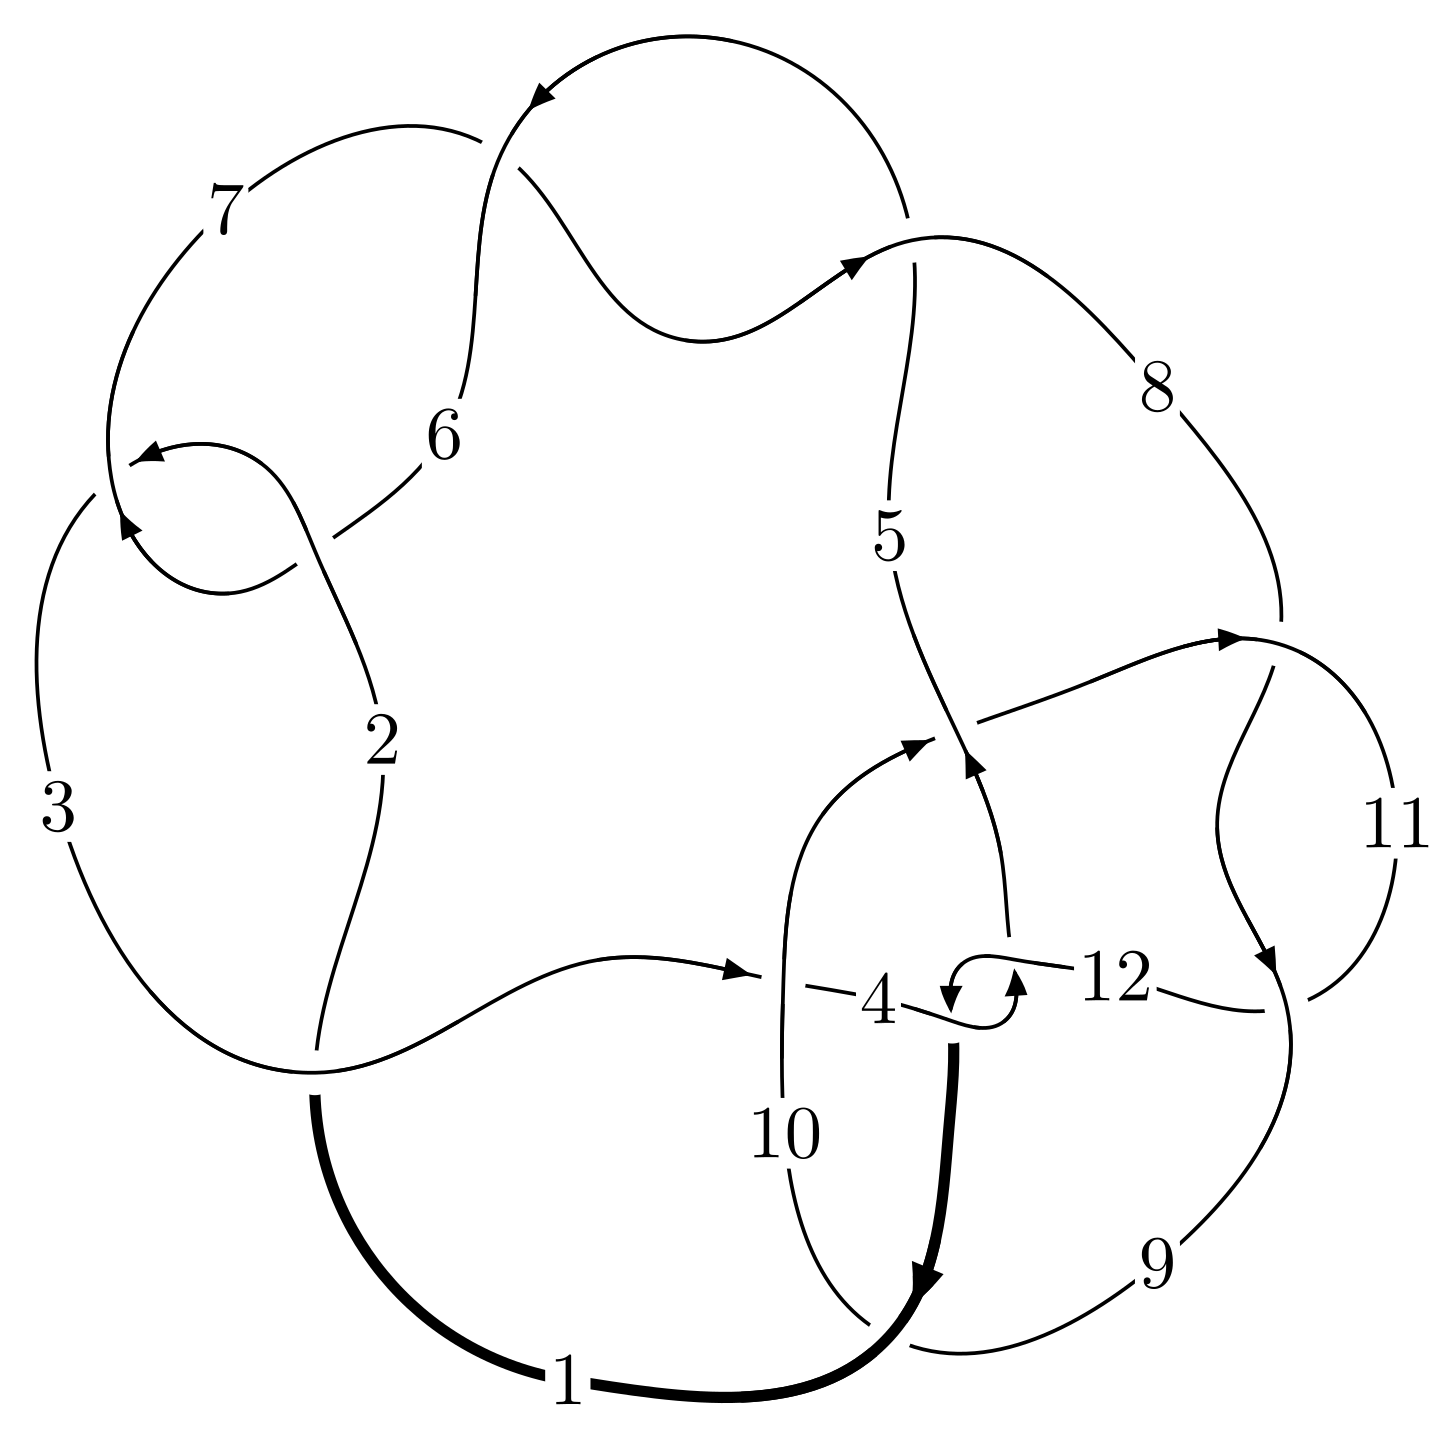
\includegraphics[width=112pt]{../../../GIT/diagram.site/Diagrams/png/1456_12a_0655.png}\\
\ \ \ A knot diagram\footnotemark}&
\allowdisplaybreaks
\textbf{Linearized knot diagam} \\
\cline{2-2}
 &
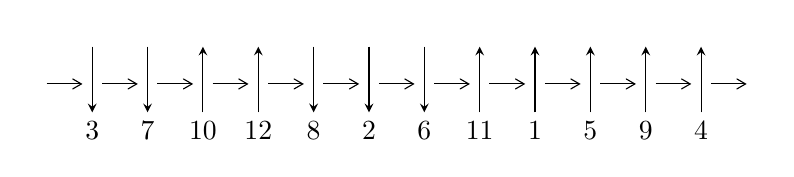
\begin{tikzpicture}[x=20pt, y=17pt]
	% nodes
	\node (C0) at (0, 0) {};
	\node (C1) at (1, 0) {};
	\node (C1U) at (1, +1) {};
	\node (C1D) at (1, -1) {3};

	\node (C2) at (2, 0) {};
	\node (C2U) at (2, +1) {};
	\node (C2D) at (2, -1) {7};

	\node (C3) at (3, 0) {};
	\node (C3U) at (3, +1) {};
	\node (C3D) at (3, -1) {10};

	\node (C4) at (4, 0) {};
	\node (C4U) at (4, +1) {};
	\node (C4D) at (4, -1) {12};

	\node (C5) at (5, 0) {};
	\node (C5U) at (5, +1) {};
	\node (C5D) at (5, -1) {8};

	\node (C6) at (6, 0) {};
	\node (C6U) at (6, +1) {};
	\node (C6D) at (6, -1) {2};

	\node (C7) at (7, 0) {};
	\node (C7U) at (7, +1) {};
	\node (C7D) at (7, -1) {6};

	\node (C8) at (8, 0) {};
	\node (C8U) at (8, +1) {};
	\node (C8D) at (8, -1) {11};

	\node (C9) at (9, 0) {};
	\node (C9U) at (9, +1) {};
	\node (C9D) at (9, -1) {1};

	\node (C10) at (10, 0) {};
	\node (C10U) at (10, +1) {};
	\node (C10D) at (10, -1) {5};

	\node (C11) at (11, 0) {};
	\node (C11U) at (11, +1) {};
	\node (C11D) at (11, -1) {9};

	\node (C12) at (12, 0) {};
	\node (C12U) at (12, +1) {};
	\node (C12D) at (12, -1) {4};
	\node (C13) at (13, 0) {};

	% arrows
	\draw[->,>={angle 60}]
	(C0) edge (C1) (C1) edge (C2) (C2) edge (C3) (C3) edge (C4) (C4) edge (C5) (C5) edge (C6) (C6) edge (C7) (C7) edge (C8) (C8) edge (C9) (C9) edge (C10) (C10) edge (C11) (C11) edge (C12) (C12) edge (C13) ;	\draw[->,>=stealth]
	(C1U) edge (C1D) (C2U) edge (C2D) (C3D) edge (C3U) (C4D) edge (C4U) (C5U) edge (C5D) (C6U) edge (C6D) (C7U) edge (C7D) (C8D) edge (C8U) (C9D) edge (C9U) (C10D) edge (C10U) (C11D) edge (C11U) (C12D) edge (C12U) ;
	\end{tikzpicture} \\
\hhline{~~} \\& 
\textbf{Solving Sequence} \\ \cline{2-2} 
 &
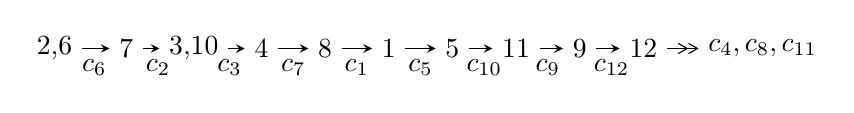
\begin{tikzpicture}[x=23pt, y=7pt]
	% node
	\node (A0) at (-1/8, 0) {2,6};
	\node (A1) at (1, 0) {7};
	\node (A2) at (33/16, 0) {3,10};
	\node (A3) at (25/8, 0) {4};
	\node (A4) at (33/8, 0) {8};
	\node (A5) at (41/8, 0) {1};
	\node (A6) at (49/8, 0) {5};
	\node (A7) at (57/8, 0) {11};
	\node (A8) at (65/8, 0) {9};
	\node (A9) at (73/8, 0) {12};
	\node (C1) at (1/2, -1) {$c_{6}$};
	\node (C2) at (3/2, -1) {$c_{2}$};
	\node (C3) at (21/8, -1) {$c_{3}$};
	\node (C4) at (29/8, -1) {$c_{7}$};
	\node (C5) at (37/8, -1) {$c_{1}$};
	\node (C6) at (45/8, -1) {$c_{5}$};
	\node (C7) at (53/8, -1) {$c_{10}$};
	\node (C8) at (61/8, -1) {$c_{9}$};
	\node (C9) at (69/8, -1) {$c_{12}$};
	\node (A10) at (11, 0) {$c_{4},c_{8},c_{11}$};

	% edge
	\draw[->,>=stealth]	
	(A0) edge (A1) (A1) edge (A2) (A2) edge (A3) (A3) edge (A4) (A4) edge (A5) (A5) edge (A6) (A6) edge (A7) (A7) edge (A8) (A8) edge (A9) ;
	\draw[->>,>={angle 60}]	
	(A9) edge (A10);
\end{tikzpicture} \\ 

\end{tabular} \\

\footnotetext{
The image of knot diagram is generated by the software ``\textbf{Draw programme}" developed by Andrew Bartholomew(\url{http://www.layer8.co.uk/maths/draw/index.htm\#Running-draw}), where we modified some parts for our purpose(\url{https://github.com/CATsTAILs/LinksPainter}).
}\phantom \\ \newline 
\centering \textbf{Ideals for irreducible components\footnotemark of $X_{\text{par}}$} 
 
\begin{align*}
I^u_{1}&=\langle 
-8.19819\times10^{42} u^{79}-1.59276\times10^{43} u^{78}+\cdots+1.35478\times10^{43} b+6.72467\times10^{42},\\
\phantom{I^u_{1}}&\phantom{= \langle  }3.41285\times10^{43} u^{79}+4.36237\times10^{43} u^{78}+\cdots+5.41912\times10^{43} a-1.57980\times10^{44},\;u^{80}+2 u^{79}+\cdots-3 u-1\rangle \\
I^u_{2}&=\langle 
b,\;2 a-1,\;u+1\rangle \\
\\
\end{align*}
\raggedright * 2 irreducible components of $\dim_{\mathbb{C}}=0$, with total 81 representations.\\
\footnotetext{All coefficients of polynomials are rational numbers. But the coefficients are sometimes approximated in decimal forms when there is not enough margin.}
\newpage
\renewcommand{\arraystretch}{1}
\centering \section*{I. $I^u_{1}= \langle -8.20\times10^{42} u^{79}-1.59\times10^{43} u^{78}+\cdots+1.35\times10^{43} b+6.72\times10^{42},\;3.41\times10^{43} u^{79}+4.36\times10^{43} u^{78}+\cdots+5.42\times10^{43} a-1.58\times10^{44},\;u^{80}+2 u^{79}+\cdots-3 u-1 \rangle$}
\flushleft \textbf{(i) Arc colorings}\\
\begin{tabular}{m{7pt} m{180pt} m{7pt} m{180pt} }
\flushright $a_{2}=$&$\begin{pmatrix}0\\u\end{pmatrix}$ \\
\flushright $a_{6}=$&$\begin{pmatrix}1\\0\end{pmatrix}$ \\
\flushright $a_{7}=$&$\begin{pmatrix}1\\u^2\end{pmatrix}$ \\
\flushright $a_{3}=$&$\begin{pmatrix}- u\\- u^3+u\end{pmatrix}$ \\
\flushright $a_{10}=$&$\begin{pmatrix}-0.629779 u^{79}-0.804997 u^{78}+\cdots-0.236236 u+2.91523\\0.605131 u^{79}+1.17566 u^{78}+\cdots+0.809601 u-0.496367\end{pmatrix}$ \\
\flushright $a_{4}=$&$\begin{pmatrix}0.0169796 u^{79}+0.335459 u^{78}+\cdots+5.83903 u+0.475568\\0.312645 u^{79}+0.279259 u^{78}+\cdots-1.22816 u-0.148293\end{pmatrix}$ \\
\flushright $a_{8}=$&$\begin{pmatrix}- u^2+1\\u^2\end{pmatrix}$ \\
\flushright $a_{1}=$&$\begin{pmatrix}u^3\\u^5- u^3+u\end{pmatrix}$ \\
\flushright $a_{5}=$&$\begin{pmatrix}u^4- u^2+1\\- u^4\end{pmatrix}$ \\
\flushright $a_{11}=$&$\begin{pmatrix}-1.02827 u^{79}-0.503727 u^{78}+\cdots+0.572706 u+2.21425\\-0.457395 u^{79}-0.709552 u^{78}+\cdots+3.16267 u+0.625862\end{pmatrix}$ \\
\flushright $a_{9}=$&$\begin{pmatrix}-0.897443 u^{79}-0.306344 u^{78}+\cdots+0.339031 u+3.14474\\-0.381766 u^{79}-0.537593 u^{78}+\cdots+3.60157 u+0.702345\end{pmatrix}$ \\
\flushright $a_{12}=$&$\begin{pmatrix}-0.148293 u^{79}+0.0160589 u^{78}+\cdots+0.773176 u-0.783280\\-0.301500 u^{79}-0.639544 u^{78}+\cdots-0.526507 u-0.0169796\end{pmatrix}$\\&\end{tabular}
\flushleft \textbf{(ii) Obstruction class $= -1$}\\~\\
\flushleft \textbf{(iii) Cusp Shapes $= -0.218530 u^{79}-4.58968 u^{78}+\cdots-13.4585 u+6.15221$}\\~\\
\newpage\renewcommand{\arraystretch}{1}
\flushleft \textbf{(iv) u-Polynomials at the component}\newline \\
\begin{tabular}{m{50pt}|m{274pt}}
Crossings & \hspace{64pt}u-Polynomials at each crossing \\
\hline $$\begin{aligned}c_{1},c_{5},c_{7}\end{aligned}$$&$\begin{aligned}
&u^{80}+18 u^{79}+\cdots+9 u+1
\end{aligned}$\\
\hline $$\begin{aligned}c_{2},c_{6}\end{aligned}$$&$\begin{aligned}
&u^{80}-2 u^{79}+\cdots+3 u-1
\end{aligned}$\\
\hline $$\begin{aligned}c_{3}\end{aligned}$$&$\begin{aligned}
&u^{80}+u^{79}+\cdots+58 u+8
\end{aligned}$\\
\hline $$\begin{aligned}c_{4},c_{12}\end{aligned}$$&$\begin{aligned}
&u^{80}+4 u^{79}+\cdots+u-1
\end{aligned}$\\
\hline $$\begin{aligned}c_{8},c_{11}\end{aligned}$$&$\begin{aligned}
&u^{80}+2 u^{79}+\cdots-23 u-4
\end{aligned}$\\
\hline $$\begin{aligned}c_{9}\end{aligned}$$&$\begin{aligned}
&2(2 u^{80}+41 u^{79}+\cdots-792 u-121)
\end{aligned}$\\
\hline $$\begin{aligned}c_{10}\end{aligned}$$&$\begin{aligned}
&2(2 u^{80}+23 u^{79}+\cdots-1532216 u+259361)
\end{aligned}$\\
\hline
\end{tabular}\\~\\
\newpage\renewcommand{\arraystretch}{1}
\flushleft \textbf{(v) Riley Polynomials at the component}\newline \\
\begin{tabular}{m{50pt}|m{274pt}}
Crossings & \hspace{64pt}Riley Polynomials at each crossing \\
\hline $$\begin{aligned}c_{1},c_{5},c_{7}\end{aligned}$$&$\begin{aligned}
&y^{80}+90 y^{79}+\cdots+23 y+1
\end{aligned}$\\
\hline $$\begin{aligned}c_{2},c_{6}\end{aligned}$$&$\begin{aligned}
&y^{80}-18 y^{79}+\cdots-9 y+1
\end{aligned}$\\
\hline $$\begin{aligned}c_{3}\end{aligned}$$&$\begin{aligned}
&y^{80}-9 y^{79}+\cdots+1228 y+64
\end{aligned}$\\
\hline $$\begin{aligned}c_{4},c_{12}\end{aligned}$$&$\begin{aligned}
&y^{80}+46 y^{79}+\cdots-9 y+1
\end{aligned}$\\
\hline $$\begin{aligned}c_{8},c_{11}\end{aligned}$$&$\begin{aligned}
&y^{80}-58 y^{79}+\cdots+1135 y+16
\end{aligned}$\\
\hline $$\begin{aligned}c_{9}\end{aligned}$$&$\begin{aligned}
&4(4 y^{80}-1149 y^{79}+\cdots-58080 y+14641)
\end{aligned}$\\
\hline $$\begin{aligned}c_{10}\end{aligned}$$&$\begin{aligned}
&4(4 y^{80}+1059 y^{79}+\cdots-1.70097\times10^{12} y+6.72681\times10^{10})
\end{aligned}$\\
\hline
\end{tabular}\\~\\
\newpage\flushleft \textbf{(vi) Complex Volumes and Cusp Shapes}
$$\begin{array}{c|c|c}  
\text{Solutions to }I^u_{1}& \I (\text{vol} + \sqrt{-1}CS) & \text{Cusp shape}\\
 \hline 
\begin{aligned}
u &= \phantom{-}0.908210 + 0.444035 I \\
a &= -1.095210 - 0.465911 I \\
b &= \phantom{-}0.438874 + 0.850544 I\end{aligned}
 & -3.55883 - 7.04654 I & \phantom{-0.000000 } 0 \\ \hline\begin{aligned}
u &= \phantom{-}0.908210 - 0.444035 I \\
a &= -1.095210 + 0.465911 I \\
b &= \phantom{-}0.438874 - 0.850544 I\end{aligned}
 & -3.55883 + 7.04654 I & \phantom{-0.000000 } 0 \\ \hline\begin{aligned}
u &= \phantom{-}0.865717 + 0.552851 I \\
a &= \phantom{-}0.875688 - 0.614993 I \\
b &= -0.389676 + 0.621158 I\end{aligned}
 & -2.62897 - 2.01090 I & \phantom{-0.000000 } 0 \\ \hline\begin{aligned}
u &= \phantom{-}0.865717 - 0.552851 I \\
a &= \phantom{-}0.875688 + 0.614993 I \\
b &= -0.389676 - 0.621158 I\end{aligned}
 & -2.62897 + 2.01090 I & \phantom{-0.000000 } 0 \\ \hline\begin{aligned}
u &= -1.029480 + 0.054908 I \\
a &= -0.086104 + 0.140911 I \\
b &= -0.611613 - 0.895210 I\end{aligned}
 & -3.03805 + 7.01781 I & \phantom{-0.000000 } 0 \\ \hline\begin{aligned}
u &= -1.029480 - 0.054908 I \\
a &= -0.086104 - 0.140911 I \\
b &= -0.611613 + 0.895210 I\end{aligned}
 & -3.03805 - 7.01781 I & \phantom{-0.000000 } 0 \\ \hline\begin{aligned}
u &= -0.862150 + 0.411938 I \\
a &= -0.765239 + 0.717847 I \\
b &= \phantom{-}0.355988 - 0.594647 I\end{aligned}
 & -0.10150 + 3.54359 I & \phantom{-0.000000 } 0. - 7.68142 I \\ \hline\begin{aligned}
u &= -0.862150 - 0.411938 I \\
a &= -0.765239 - 0.717847 I \\
b &= \phantom{-}0.355988 + 0.594647 I\end{aligned}
 & -0.10150 - 3.54359 I & \phantom{-0.000000 -}0. + 7.68142 I \\ \hline\begin{aligned}
u &= -0.805506 + 0.494428 I \\
a &= -1.054990 + 0.759347 I \\
b &= -0.414849 + 0.172313 I\end{aligned}
 & \phantom{-}1.50560 + 5.11913 I & \phantom{-}5.17837 - 10.30158 I \\ \hline\begin{aligned}
u &= -0.805506 - 0.494428 I \\
a &= -1.054990 - 0.759347 I \\
b &= -0.414849 - 0.172313 I\end{aligned}
 & \phantom{-}1.50560 - 5.11913 I & \phantom{-}5.17837 + 10.30158 I\\
 \hline 
 \end{array}$$\newpage$$\begin{array}{c|c|c}  
\text{Solutions to }I^u_{1}& \I (\text{vol} + \sqrt{-1}CS) & \text{Cusp shape}\\
 \hline 
\begin{aligned}
u &= -0.900523 + 0.041367 I \\
a &= -0.305993 - 0.178109 I \\
b &= \phantom{-}0.720582 - 1.129830 I\end{aligned}
 & -5.73822 - 2.28735 I & -7.12415 + 1.62116 I \\ \hline\begin{aligned}
u &= -0.900523 - 0.041367 I \\
a &= -0.305993 + 0.178109 I \\
b &= \phantom{-}0.720582 + 1.129830 I\end{aligned}
 & -5.73822 + 2.28735 I & -7.12415 - 1.62116 I \\ \hline\begin{aligned}
u &= -0.376173 + 0.818414 I \\
a &= -0.757603 + 0.029800 I \\
b &= \phantom{-}0.455373 - 0.302854 I\end{aligned}
 & \phantom{-}5.96762 - 1.94537 I & \phantom{-}12.19550 + 3.06031 I \\ \hline\begin{aligned}
u &= -0.376173 - 0.818414 I \\
a &= -0.757603 - 0.029800 I \\
b &= \phantom{-}0.455373 + 0.302854 I\end{aligned}
 & \phantom{-}5.96762 + 1.94537 I & \phantom{-}12.19550 - 3.06031 I \\ \hline\begin{aligned}
u &= \phantom{-}0.997813 + 0.498144 I \\
a &= \phantom{-}1.059100 + 0.742760 I \\
b &= -0.668142 - 0.394736 I\end{aligned}
 & \phantom{-}0.21830 - 12.90460 I & \phantom{-0.000000 } 0 \\ \hline\begin{aligned}
u &= \phantom{-}0.997813 - 0.498144 I \\
a &= \phantom{-}1.059100 - 0.742760 I \\
b &= -0.668142 + 0.394736 I\end{aligned}
 & \phantom{-}0.21830 + 12.90460 I & \phantom{-0.000000 } 0 \\ \hline\begin{aligned}
u &= \phantom{-}0.736410 + 0.485024 I \\
a &= -0.962764 - 0.238510 I \\
b &= -0.258198 - 1.145200 I\end{aligned}
 & \phantom{-}2.76606 - 1.97173 I & \phantom{-}7.71264 + 2.63546 I \\ \hline\begin{aligned}
u &= \phantom{-}0.736410 - 0.485024 I \\
a &= -0.962764 + 0.238510 I \\
b &= -0.258198 + 1.145200 I\end{aligned}
 & \phantom{-}2.76606 + 1.97173 I & \phantom{-}7.71264 - 2.63546 I \\ \hline\begin{aligned}
u &= \phantom{-}1.065740 + 0.394552 I \\
a &= -0.227830 + 0.296596 I \\
b &= \phantom{-}0.262901 + 0.085388 I\end{aligned}
 & -1.036590 + 0.614054 I & \phantom{-0.000000 } 0 \\ \hline\begin{aligned}
u &= \phantom{-}1.065740 - 0.394552 I \\
a &= -0.227830 - 0.296596 I \\
b &= \phantom{-}0.262901 - 0.085388 I\end{aligned}
 & -1.036590 - 0.614054 I & \phantom{-0.000000 } 0\\
 \hline 
 \end{array}$$\newpage$$\begin{array}{c|c|c}  
\text{Solutions to }I^u_{1}& \I (\text{vol} + \sqrt{-1}CS) & \text{Cusp shape}\\
 \hline 
\begin{aligned}
u &= \phantom{-}0.393317 + 0.768055 I \\
a &= -1.219110 - 0.511536 I \\
b &= \phantom{-}0.585050 + 0.524028 I\end{aligned}
 & \phantom{-}2.20503 + 8.30381 I & \phantom{-}6.33496 - 5.30249 I \\ \hline\begin{aligned}
u &= \phantom{-}0.393317 - 0.768055 I \\
a &= -1.219110 + 0.511536 I \\
b &= \phantom{-}0.585050 - 0.524028 I\end{aligned}
 & \phantom{-}2.20503 - 8.30381 I & \phantom{-}6.33496 + 5.30249 I \\ \hline\begin{aligned}
u &= -1.024360 + 0.515111 I \\
a &= \phantom{-}0.624975 - 0.528092 I \\
b &= -0.311319 + 0.219577 I\end{aligned}
 & \phantom{-}3.83148 + 6.74819 I & \phantom{-0.000000 } 0 \\ \hline\begin{aligned}
u &= -1.024360 - 0.515111 I \\
a &= \phantom{-}0.624975 + 0.528092 I \\
b &= -0.311319 - 0.219577 I\end{aligned}
 & \phantom{-}3.83148 - 6.74819 I & \phantom{-0.000000 } 0 \\ \hline\begin{aligned}
u &= \phantom{-}0.687160 + 0.501005 I \\
a &= -0.282184 - 0.064378 I \\
b &= -0.51019 - 1.36518 I\end{aligned}
 & \phantom{-}2.92099 - 1.83327 I & \phantom{-}8.18864 + 5.75972 I \\ \hline\begin{aligned}
u &= \phantom{-}0.687160 - 0.501005 I \\
a &= -0.282184 + 0.064378 I \\
b &= -0.51019 + 1.36518 I\end{aligned}
 & \phantom{-}2.92099 + 1.83327 I & \phantom{-}8.18864 - 5.75972 I \\ \hline\begin{aligned}
u &= -0.769360 + 0.358403 I \\
a &= -2.31120 + 5.45588 I \\
b &= \phantom{-}3.99649 - 1.94508 I\end{aligned}
 & -0.280690 + 1.300660 I & \phantom{-}18.3751 - 32.3353 I \\ \hline\begin{aligned}
u &= -0.769360 - 0.358403 I \\
a &= -2.31120 - 5.45588 I \\
b &= \phantom{-}3.99649 + 1.94508 I\end{aligned}
 & -0.280690 - 1.300660 I & \phantom{-}18.3751 + 32.3353 I \\ \hline\begin{aligned}
u &= \phantom{-}0.819942 + 0.191250 I \\
a &= \phantom{-}0.078129 - 0.134282 I \\
b &= \phantom{-}0.356444 + 0.554305 I\end{aligned}
 & -1.40523 - 0.61914 I & -4.60800 + 0.82851 I \\ \hline\begin{aligned}
u &= \phantom{-}0.819942 - 0.191250 I \\
a &= \phantom{-}0.078129 + 0.134282 I \\
b &= \phantom{-}0.356444 - 0.554305 I\end{aligned}
 & -1.40523 + 0.61914 I & -4.60800 - 0.82851 I\\
 \hline 
 \end{array}$$\newpage$$\begin{array}{c|c|c}  
\text{Solutions to }I^u_{1}& \I (\text{vol} + \sqrt{-1}CS) & \text{Cusp shape}\\
 \hline 
\begin{aligned}
u &= \phantom{-}1.16108\phantom{ +0.000000I} \\
a &= -0.0517082\phantom{ +0.000000I} \\
b &= -0.378668\phantom{ +0.000000I}\end{aligned}
 & \phantom{-}0.324488\phantom{ +0.000000I} & \phantom{-0.000000 } 0 \\ \hline\begin{aligned}
u &= \phantom{-}0.276198 + 0.789141 I \\
a &= -0.201775 + 0.641459 I \\
b &= \phantom{-}0.394592 - 0.012771 I\end{aligned}
 & \phantom{-}1.64531 - 4.95419 I & \phantom{-}7.71109 + 7.25315 I \\ \hline\begin{aligned}
u &= \phantom{-}0.276198 - 0.789141 I \\
a &= -0.201775 - 0.641459 I \\
b &= \phantom{-}0.394592 + 0.012771 I\end{aligned}
 & \phantom{-}1.64531 + 4.95419 I & \phantom{-}7.71109 - 7.25315 I \\ \hline\begin{aligned}
u &= -0.594052 + 0.518671 I \\
a &= \phantom{-}0.926803 + 0.177997 I \\
b &= -0.441308 + 1.081290 I\end{aligned}
 & \phantom{-}2.16348 - 1.21726 I & \phantom{-}8.19465 + 1.97536 I \\ \hline\begin{aligned}
u &= -0.594052 - 0.518671 I \\
a &= \phantom{-}0.926803 - 0.177997 I \\
b &= -0.441308 - 1.081290 I\end{aligned}
 & \phantom{-}2.16348 + 1.21726 I & \phantom{-}8.19465 - 1.97536 I \\ \hline\begin{aligned}
u &= -0.888871 + 0.850062 I \\
a &= -1.031000 + 0.156735 I \\
b &= \phantom{-}0.81250 + 1.39597 I\end{aligned}
 & \phantom{-}5.01781 + 2.94177 I & \phantom{-0.000000 } 0 \\ \hline\begin{aligned}
u &= -0.888871 - 0.850062 I \\
a &= -1.031000 - 0.156735 I \\
b &= \phantom{-}0.81250 - 1.39597 I\end{aligned}
 & \phantom{-}5.01781 - 2.94177 I & \phantom{-0.000000 } 0 \\ \hline\begin{aligned}
u &= \phantom{-}0.884877 + 0.875922 I \\
a &= -1.64030 - 1.54748 I \\
b &= \phantom{-}3.03145 - 0.58809 I\end{aligned}
 & \phantom{-}7.91819 - 0.07865 I & \phantom{-0.000000 } 0 \\ \hline\begin{aligned}
u &= \phantom{-}0.884877 - 0.875922 I \\
a &= -1.64030 + 1.54748 I \\
b &= \phantom{-}3.03145 + 0.58809 I\end{aligned}
 & \phantom{-}7.91819 + 0.07865 I & \phantom{-0.000000 } 0 \\ \hline\begin{aligned}
u &= -0.926943 + 0.832833 I \\
a &= \phantom{-}0.286660 - 0.815402 I \\
b &= -1.52828 + 0.64200 I\end{aligned}
 & \phantom{-}4.89547 + 3.32207 I & \phantom{-0.000000 } 0\\
 \hline 
 \end{array}$$\newpage$$\begin{array}{c|c|c}  
\text{Solutions to }I^u_{1}& \I (\text{vol} + \sqrt{-1}CS) & \text{Cusp shape}\\
 \hline 
\begin{aligned}
u &= -0.926943 - 0.832833 I \\
a &= \phantom{-}0.286660 + 0.815402 I \\
b &= -1.52828 - 0.64200 I\end{aligned}
 & \phantom{-}4.89547 - 3.32207 I & \phantom{-0.000000 } 0 \\ \hline\begin{aligned}
u &= -0.875865 + 0.887015 I \\
a &= -1.21431 + 2.34469 I \\
b &= \phantom{-}3.30413 - 0.59349 I\end{aligned}
 & \phantom{-}4.89656 - 3.73236 I & \phantom{-0.000000 } 0 \\ \hline\begin{aligned}
u &= -0.875865 - 0.887015 I \\
a &= -1.21431 - 2.34469 I \\
b &= \phantom{-}3.30413 + 0.59349 I\end{aligned}
 & \phantom{-}4.89656 + 3.73236 I & \phantom{-0.000000 } 0 \\ \hline\begin{aligned}
u &= \phantom{-}0.913469 + 0.855850 I \\
a &= \phantom{-}7.90543 - 5.83238 I \\
b &= \phantom{-}2.1500 + 17.7012 I\end{aligned}
 & \phantom{-}6.83434 - 3.17732 I & \phantom{-0.000000 } 0 \\ \hline\begin{aligned}
u &= \phantom{-}0.913469 - 0.855850 I \\
a &= \phantom{-}7.90543 + 5.83238 I \\
b &= \phantom{-}2.1500 - 17.7012 I\end{aligned}
 & \phantom{-}6.83434 + 3.17732 I & \phantom{-0.000000 } 0 \\ \hline\begin{aligned}
u &= -0.858554 + 0.925077 I \\
a &= \phantom{-}1.36360 - 1.87978 I \\
b &= -3.18932 + 0.02579 I\end{aligned}
 & \phantom{-}9.7035 - 10.2935 I & \phantom{-0.000000 } 0 \\ \hline\begin{aligned}
u &= -0.858554 - 0.925077 I \\
a &= \phantom{-}1.36360 + 1.87978 I \\
b &= -3.18932 - 0.02579 I\end{aligned}
 & \phantom{-}9.7035 + 10.2935 I & \phantom{-0.000000 } 0 \\ \hline\begin{aligned}
u &= \phantom{-}0.905807 + 0.883629 I \\
a &= -2.49473 - 0.75276 I \\
b &= \phantom{-}3.27476 - 1.66368 I\end{aligned}
 & \phantom{-}9.90082 + 0.66319 I & \phantom{-0.000000 } 0 \\ \hline\begin{aligned}
u &= \phantom{-}0.905807 - 0.883629 I \\
a &= -2.49473 + 0.75276 I \\
b &= \phantom{-}3.27476 + 1.66368 I\end{aligned}
 & \phantom{-}9.90082 - 0.66319 I & \phantom{-0.000000 } 0 \\ \hline\begin{aligned}
u &= \phantom{-}0.723920 + 0.124460 I \\
a &= \phantom{-}1.21857 - 1.47110 I \\
b &= \phantom{-}0.780068 + 0.970212 I\end{aligned}
 & -1.21288 - 2.12033 I & -2.81970 + 3.07552 I\\
 \hline 
 \end{array}$$\newpage$$\begin{array}{c|c|c}  
\text{Solutions to }I^u_{1}& \I (\text{vol} + \sqrt{-1}CS) & \text{Cusp shape}\\
 \hline 
\begin{aligned}
u &= \phantom{-}0.723920 - 0.124460 I \\
a &= \phantom{-}1.21857 + 1.47110 I \\
b &= \phantom{-}0.780068 - 0.970212 I\end{aligned}
 & -1.21288 + 2.12033 I & -2.81970 - 3.07552 I \\ \hline\begin{aligned}
u &= \phantom{-}0.857297 + 0.932255 I \\
a &= \phantom{-}1.30613 + 1.32110 I \\
b &= -2.54938 + 0.28745 I\end{aligned}
 & \phantom{-}13.5592 + 4.2838 I & \phantom{-0.000000 } 0 \\ \hline\begin{aligned}
u &= \phantom{-}0.857297 - 0.932255 I \\
a &= \phantom{-}1.30613 - 1.32110 I \\
b &= -2.54938 - 0.28745 I\end{aligned}
 & \phantom{-}13.5592 - 4.2838 I & \phantom{-0.000000 } 0 \\ \hline\begin{aligned}
u &= -0.916009 + 0.877875 I \\
a &= -1.376650 - 0.243211 I \\
b &= \phantom{-}1.47545 + 1.19753 I\end{aligned}
 & \phantom{-}10.84760 + 2.95253 I & \phantom{-0.000000 } 0 \\ \hline\begin{aligned}
u &= -0.916009 - 0.877875 I \\
a &= -1.376650 + 0.243211 I \\
b &= \phantom{-}1.47545 - 1.19753 I\end{aligned}
 & \phantom{-}10.84760 - 2.95253 I & \phantom{-0.000000 } 0 \\ \hline\begin{aligned}
u &= \phantom{-}0.945271 + 0.851052 I \\
a &= \phantom{-}1.65910 + 1.44872 I \\
b &= -3.28901 + 0.49671 I\end{aligned}
 & \phantom{-}7.72695 - 6.32210 I & \phantom{-0.000000 } 0 \\ \hline\begin{aligned}
u &= \phantom{-}0.945271 - 0.851052 I \\
a &= \phantom{-}1.65910 - 1.44872 I \\
b &= -3.28901 - 0.49671 I\end{aligned}
 & \phantom{-}7.72695 + 6.32210 I & \phantom{-0.000000 } 0 \\ \hline\begin{aligned}
u &= -0.926203 + 0.873253 I \\
a &= -0.00593 - 1.47214 I \\
b &= -1.146450 + 0.764895 I\end{aligned}
 & \phantom{-}10.81490 + 3.52603 I & \phantom{-0.000000 } 0 \\ \hline\begin{aligned}
u &= -0.926203 - 0.873253 I \\
a &= -0.00593 + 1.47214 I \\
b &= -1.146450 - 0.764895 I\end{aligned}
 & \phantom{-}10.81490 - 3.52603 I & \phantom{-0.000000 } 0 \\ \hline\begin{aligned}
u &= \phantom{-}0.936906 + 0.870026 I \\
a &= \phantom{-}1.02403 + 2.45543 I \\
b &= -3.30105 - 0.80227 I\end{aligned}
 & \phantom{-}9.80182 - 7.14932 I & \phantom{-0.000000 } 0\\
 \hline 
 \end{array}$$\newpage$$\begin{array}{c|c|c}  
\text{Solutions to }I^u_{1}& \I (\text{vol} + \sqrt{-1}CS) & \text{Cusp shape}\\
 \hline 
\begin{aligned}
u &= \phantom{-}0.936906 - 0.870026 I \\
a &= \phantom{-}1.02403 - 2.45543 I \\
b &= -3.30105 + 0.80227 I\end{aligned}
 & \phantom{-}9.80182 + 7.14932 I & \phantom{-0.000000 } 0 \\ \hline\begin{aligned}
u &= -0.847914 + 0.957867 I \\
a &= \phantom{-}0.799931 - 0.479515 I \\
b &= -1.283290 - 0.364046 I\end{aligned}
 & \phantom{-}8.58054 + 1.91116 I & \phantom{-0.000000 } 0 \\ \hline\begin{aligned}
u &= -0.847914 - 0.957867 I \\
a &= \phantom{-}0.799931 + 0.479515 I \\
b &= -1.283290 + 0.364046 I\end{aligned}
 & \phantom{-}8.58054 - 1.91116 I & \phantom{-0.000000 } 0 \\ \hline\begin{aligned}
u &= -0.957274 + 0.852492 I \\
a &= \phantom{-}2.41489 - 0.96433 I \\
b &= -3.42506 - 1.60897 I\end{aligned}
 & \phantom{-}4.63845 + 10.17100 I & \phantom{-0.000000 } 0 \\ \hline\begin{aligned}
u &= -0.957274 - 0.852492 I \\
a &= \phantom{-}2.41489 + 0.96433 I \\
b &= -3.42506 + 1.60897 I\end{aligned}
 & \phantom{-}4.63845 - 10.17100 I & \phantom{-0.000000 } 0 \\ \hline\begin{aligned}
u &= \phantom{-}0.484225 + 0.490550 I \\
a &= \phantom{-}0.85564 - 1.37009 I \\
b &= -0.190985 + 0.748669 I\end{aligned}
 & -1.75610 - 2.02511 I & \phantom{-}1.63204 + 3.32753 I \\ \hline\begin{aligned}
u &= \phantom{-}0.484225 - 0.490550 I \\
a &= \phantom{-}0.85564 + 1.37009 I \\
b &= -0.190985 - 0.748669 I\end{aligned}
 & -1.75610 + 2.02511 I & \phantom{-}1.63204 - 3.32753 I \\ \hline\begin{aligned}
u &= -0.989525 + 0.860769 I \\
a &= -1.97327 + 1.20741 I \\
b &= \phantom{-}3.46394 + 1.15460 I\end{aligned}
 & \phantom{-}9.2811 + 16.8739 I & \phantom{-0.000000 } 0 \\ \hline\begin{aligned}
u &= -0.989525 - 0.860769 I \\
a &= -1.97327 - 1.20741 I \\
b &= \phantom{-}3.46394 - 1.15460 I\end{aligned}
 & \phantom{-}9.2811 - 16.8739 I & \phantom{-0.000000 } 0 \\ \hline\begin{aligned}
u &= \phantom{-}0.994452 + 0.863666 I \\
a &= -1.45453 - 1.16136 I \\
b &= \phantom{-}2.82195 - 0.59826 I\end{aligned}
 & \phantom{-}13.1160 - 10.8953 I & \phantom{-0.000000 } 0\\
 \hline 
 \end{array}$$\newpage$$\begin{array}{c|c|c}  
\text{Solutions to }I^u_{1}& \I (\text{vol} + \sqrt{-1}CS) & \text{Cusp shape}\\
 \hline 
\begin{aligned}
u &= \phantom{-}0.994452 - 0.863666 I \\
a &= -1.45453 + 1.16136 I \\
b &= \phantom{-}2.82195 + 0.59826 I\end{aligned}
 & \phantom{-}13.1160 + 10.8953 I & \phantom{-0.000000 } 0 \\ \hline\begin{aligned}
u &= \phantom{-}0.379240 + 0.558264 I \\
a &= \phantom{-}1.51378 + 0.48363 I \\
b &= \phantom{-}0.013302 - 0.381211 I\end{aligned}
 & -1.97201 + 3.24293 I & \phantom{-}2.89878 - 3.45469 I \\ \hline\begin{aligned}
u &= \phantom{-}0.379240 - 0.558264 I \\
a &= \phantom{-}1.51378 - 0.48363 I \\
b &= \phantom{-}0.013302 + 0.381211 I\end{aligned}
 & -1.97201 - 3.24293 I & \phantom{-}2.89878 + 3.45469 I \\ \hline\begin{aligned}
u &= -1.013580 + 0.875810 I \\
a &= -0.681351 + 0.629833 I \\
b &= \phantom{-}1.370530 + 0.267728 I\end{aligned}
 & \phantom{-}8.04920 + 4.81399 I & \phantom{-0.000000 } 0 \\ \hline\begin{aligned}
u &= -1.013580 - 0.875810 I \\
a &= -0.681351 - 0.629833 I \\
b &= \phantom{-}1.370530 - 0.267728 I\end{aligned}
 & \phantom{-}8.04920 - 4.81399 I & \phantom{-0.000000 } 0 \\ \hline\begin{aligned}
u &= -0.449816 + 0.406846 I \\
a &= \phantom{-}1.48792 - 0.04382 I \\
b &= -0.402780 + 0.191398 I\end{aligned}
 & \phantom{-}1.139930 - 0.176228 I & \phantom{-}8.91211 + 0.28630 I \\ \hline\begin{aligned}
u &= -0.449816 - 0.406846 I \\
a &= \phantom{-}1.48792 + 0.04382 I \\
b &= -0.402780 - 0.191398 I\end{aligned}
 & \phantom{-}1.139930 + 0.176228 I & \phantom{-}8.91211 - 0.28630 I \\ \hline\begin{aligned}
u &= -0.436460\phantom{ +0.000000I} \\
a &= \phantom{-}2.21751\phantom{ +0.000000I} \\
b &= -0.515297\phantom{ +0.000000I}\end{aligned}
 & \phantom{-}1.05778\phantom{ +0.000000I} & \phantom{-}11.1780\phantom{ +0.000000I} \\ \hline\begin{aligned}
u &= -0.126130 + 0.299152 I \\
a &= \phantom{-}3.40879 + 0.64147 I \\
b &= -1.206450 - 0.292678 I\end{aligned}
 & \phantom{-}0.958209 + 1.026080 I & \phantom{-}4.35377 + 0.66475 I \\ \hline\begin{aligned}
u &= -0.126130 - 0.299152 I \\
a &= \phantom{-}3.40879 - 0.64147 I \\
b &= -1.206450 + 0.292678 I\end{aligned}
 & \phantom{-}0.958209 - 1.026080 I & \phantom{-}4.35377 - 0.66475 I\\
 \hline 
 \end{array}$$\newpage\newpage\renewcommand{\arraystretch}{1}
\centering \section*{II. $I^u_{2}= \langle b,\;2 a-1,\;u+1 \rangle$}
\flushleft \textbf{(i) Arc colorings}\\
\begin{tabular}{m{7pt} m{180pt} m{7pt} m{180pt} }
\flushright $a_{2}=$&$\begin{pmatrix}0\\-1\end{pmatrix}$ \\
\flushright $a_{6}=$&$\begin{pmatrix}1\\0\end{pmatrix}$ \\
\flushright $a_{7}=$&$\begin{pmatrix}1\\1\end{pmatrix}$ \\
\flushright $a_{3}=$&$\begin{pmatrix}1\\0\end{pmatrix}$ \\
\flushright $a_{10}=$&$\begin{pmatrix}0.5\\0\end{pmatrix}$ \\
\flushright $a_{4}=$&$\begin{pmatrix}1\\0\end{pmatrix}$ \\
\flushright $a_{8}=$&$\begin{pmatrix}0\\1\end{pmatrix}$ \\
\flushright $a_{1}=$&$\begin{pmatrix}-1\\-1\end{pmatrix}$ \\
\flushright $a_{5}=$&$\begin{pmatrix}1\\-1\end{pmatrix}$ \\
\flushright $a_{11}=$&$\begin{pmatrix}1\\-0.5\end{pmatrix}$ \\
\flushright $a_{9}=$&$\begin{pmatrix}1\\0.5\end{pmatrix}$ \\
\flushright $a_{12}=$&$\begin{pmatrix}0\\-1\end{pmatrix}$\\&\end{tabular}
\flushleft \textbf{(ii) Obstruction class $= 1$}\\~\\
\flushleft \textbf{(iii) Cusp Shapes $= -2.25$}\\~\\
\newpage\renewcommand{\arraystretch}{1}
\flushleft \textbf{(iv) u-Polynomials at the component}\newline \\
\begin{tabular}{m{50pt}|m{274pt}}
Crossings & \hspace{64pt}u-Polynomials at each crossing \\
\hline $$\begin{aligned}c_{1},c_{2},c_{5}\\c_{11},c_{12}\end{aligned}$$&$\begin{aligned}
&u-1
\end{aligned}$\\
\hline $$\begin{aligned}c_{3}\end{aligned}$$&$\begin{aligned}
&u
\end{aligned}$\\
\hline $$\begin{aligned}c_{4},c_{6},c_{7}\\c_{8}\end{aligned}$$&$\begin{aligned}
&u+1
\end{aligned}$\\
\hline $$\begin{aligned}c_{9},c_{10}\end{aligned}$$&$\begin{aligned}
&2(2 u+1)
\end{aligned}$\\
\hline
\end{tabular}\\~\\
\newpage\renewcommand{\arraystretch}{1}
\flushleft \textbf{(v) Riley Polynomials at the component}\newline \\
\begin{tabular}{m{50pt}|m{274pt}}
Crossings & \hspace{64pt}Riley Polynomials at each crossing \\
\hline $$\begin{aligned}c_{1},c_{2},c_{4}\\c_{5},c_{6},c_{7}\\c_{8},c_{11},c_{12}\end{aligned}$$&$\begin{aligned}
&y-1
\end{aligned}$\\
\hline $$\begin{aligned}c_{3}\end{aligned}$$&$\begin{aligned}
&y
\end{aligned}$\\
\hline $$\begin{aligned}c_{9},c_{10}\end{aligned}$$&$\begin{aligned}
&4(4 y-1)
\end{aligned}$\\
\hline
\end{tabular}\\~\\
\newpage\flushleft \textbf{(vi) Complex Volumes and Cusp Shapes}
$$\begin{array}{c|c|c}  
\text{Solutions to }I^u_{2}& \I (\text{vol} + \sqrt{-1}CS) & \text{Cusp shape}\\
 \hline 
\begin{aligned}
u &= -1.00000\phantom{ +0.000000I} \\
a &= \phantom{-}0.500000\phantom{ +0.000000I} \\
b &= \phantom{-0.000000 } 0\end{aligned}
 & \phantom{-0.000000 } 0 & -2.25000\phantom{ +0.000000I}\\
 \hline 
 \end{array}$$\newpage
\newpage\renewcommand{\arraystretch}{1}
\centering \section*{ III. u-Polynomials}
\begin{tabular}{m{50pt}|m{274pt}}
Crossings & \hspace{64pt}u-Polynomials at each crossing \\
\hline $$\begin{aligned}c_{1},c_{5}\end{aligned}$$&$\begin{aligned}
&(u-1)(u^{80}+18 u^{79}+\cdots+9 u+1)
\end{aligned}$\\
\hline $$\begin{aligned}c_{2}\end{aligned}$$&$\begin{aligned}
&(u-1)(u^{80}-2 u^{79}+\cdots+3 u-1)
\end{aligned}$\\
\hline $$\begin{aligned}c_{3}\end{aligned}$$&$\begin{aligned}
&u(u^{80}+u^{79}+\cdots+58 u+8)
\end{aligned}$\\
\hline $$\begin{aligned}c_{4}\end{aligned}$$&$\begin{aligned}
&(u+1)(u^{80}+4 u^{79}+\cdots+u-1)
\end{aligned}$\\
\hline $$\begin{aligned}c_{6}\end{aligned}$$&$\begin{aligned}
&(u+1)(u^{80}-2 u^{79}+\cdots+3 u-1)
\end{aligned}$\\
\hline $$\begin{aligned}c_{7}\end{aligned}$$&$\begin{aligned}
&(u+1)(u^{80}+18 u^{79}+\cdots+9 u+1)
\end{aligned}$\\
\hline $$\begin{aligned}c_{8}\end{aligned}$$&$\begin{aligned}
&(u+1)(u^{80}+2 u^{79}+\cdots-23 u-4)
\end{aligned}$\\
\hline $$\begin{aligned}c_{9}\end{aligned}$$&$\begin{aligned}
&4(2 u+1)(2 u^{80}+41 u^{79}+\cdots-792 u-121)
\end{aligned}$\\
\hline $$\begin{aligned}c_{10}\end{aligned}$$&$\begin{aligned}
&4(2 u+1)(2 u^{80}+23 u^{79}+\cdots-1532216 u+259361)
\end{aligned}$\\
\hline $$\begin{aligned}c_{11}\end{aligned}$$&$\begin{aligned}
&(u-1)(u^{80}+2 u^{79}+\cdots-23 u-4)
\end{aligned}$\\
\hline $$\begin{aligned}c_{12}\end{aligned}$$&$\begin{aligned}
&(u-1)(u^{80}+4 u^{79}+\cdots+u-1)
\end{aligned}$\\
\hline
\end{tabular}\newpage\renewcommand{\arraystretch}{1}
\centering \section*{ IV. Riley Polynomials}
\begin{tabular}{m{50pt}|m{274pt}}
Crossings & \hspace{64pt}Riley Polynomials at each crossing \\
\hline $$\begin{aligned}c_{1},c_{5},c_{7}\end{aligned}$$&$\begin{aligned}
&(y-1)(y^{80}+90 y^{79}+\cdots+23 y+1)
\end{aligned}$\\
\hline $$\begin{aligned}c_{2},c_{6}\end{aligned}$$&$\begin{aligned}
&(y-1)(y^{80}-18 y^{79}+\cdots-9 y+1)
\end{aligned}$\\
\hline $$\begin{aligned}c_{3}\end{aligned}$$&$\begin{aligned}
&y(y^{80}-9 y^{79}+\cdots+1228 y+64)
\end{aligned}$\\
\hline $$\begin{aligned}c_{4},c_{12}\end{aligned}$$&$\begin{aligned}
&(y-1)(y^{80}+46 y^{79}+\cdots-9 y+1)
\end{aligned}$\\
\hline $$\begin{aligned}c_{8},c_{11}\end{aligned}$$&$\begin{aligned}
&(y-1)(y^{80}-58 y^{79}+\cdots+1135 y+16)
\end{aligned}$\\
\hline $$\begin{aligned}c_{9}\end{aligned}$$&$\begin{aligned}
&16(4 y-1)(4 y^{80}-1149 y^{79}+\cdots-58080 y+14641)
\end{aligned}$\\
\hline $$\begin{aligned}c_{10}\end{aligned}$$&$\begin{aligned}
&16(4 y-1)\\
&\cdot(4 y^{80}+1059 y^{79}+\cdots-1700965067380 y+67268128321)
\end{aligned}$\\
\hline
\end{tabular}
\vskip 2pc
\end{document}